%Author Alex Clemmer
%CS 3100 Models of Computation
%Assignment 9:
\documentclass[a4paper]{article}
\usepackage[pdftex]{graphicx}
\usepackage{fancyvrb}
\usepackage{multirow}
\usepackage{amssymb}
\usepackage{amsmath}
\usepackage{fullpage}
\addtolength{\oddsidemargin}{-.05in}
	\addtolength{\evensidemargin}{-.05in}
	\addtolength{\textwidth}{.25in}

	\addtolength{\textheight}{.25in}

\begin{document}

\section*{Assignment 9}
Alex Clemmer\\
CS 3100 \\
Student number: u0458675

\subsection*{Problem 1:}

This minimization is pretty simple:

\begin{verbatim}
2 .         2 x         2 x         2 x
3 . .       3 x .       3 x x       3 x x
4 . . .     4 x . .     4 x x .     4 x x .
  1 2 3     1 2 3       1 2 3       1 2 3       
\end{verbatim}

Thus states 3 and 4 get merged. We end up with a 3-state FA: 1 and 2 do not change, but 3 and 4 are merged into one state. This works because 3 and 4 both point to state 4 on a $\texttt{1}$ and state 2 on a $\texttt{0}$. Thus this merged hybrid state ends up moving to state 2 on a $\texttt{0}$ and itself on a $\texttt{1}$. Further, the only way to get to it is to move from state 2 into it using an input of $\texttt{1}$.

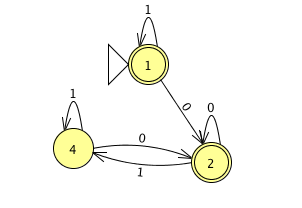
\includegraphics[scale=0.60]{1_DFA.png}

\subsection*{Problem 2:} 

Really, the simplest way we can conclude that both halves of 10.13 are equivalent is by using the method of transformation from the last question. That is, we can just look at the DFAs and compare them to find out they're isomorphic.

There are of course requisite checks we can run: they have the same number of states, and further, the same number of both final and non-final states, both of which are required for true equivalence. Then, looking at each in sequence starting from the top reveals that there is an equivalent state for each. In other words, for starters, we can conclude that they're isomorphic simply by looking at the machines (which is what we really did in the last problem).

The biggest obstacle in this case is that the layout of the two graphs does not $\textit{prima facie}$ look that similar. Yet a closer inspection reveals that this is not the case: they in fact are isomorphic. As for actually listing their equivalent states between the two machines, the isomorphic relationship can be described as follows (numbers on the left corresponding to the left part of 10.13, and numbers on the right corresponding to the right part of 10.13):

\begin{equation}
\texttt{8->10; 11->11; 6->7; 12->12; 9->9; 10->6; 7->8; 4->1; 2->3; 3->2; 0->4; 5->0; 1->5}
\end{equation}

\subsection*{Problem 3:}

Given some FA, say we replace every symbol in its alphabet with $\{a\}$. This in all cases except the most simple DFAs gives us a $\textit{strictly}$ nondeterministic FA (since it is impossible to have many choices going to different states using the same letter). This resulting NFA gives us strings that are the same $\textit{length}$ as the strings generated by the original NFA.

Now, the interesting part. If we transform our new NFA into a DFA, the machine for all non-trivial cases ends up coiling into itself (and the trivial cases will extend our conclusion, as we will see shortly). So why is this?

On a very high level, remember that this NFA is essentially measuring the lengths of the strings of some regular expression. The impact of this is that the lengths of strings ends up being the product of some set of fixed length (sub-)expressions. In other words, in contrast with context-free languages, which can be recursively variable-length ($\textit{e.g.}$, $\{0^n 1^n\}$, whose second half length is defined by the length of the first half, as opposed to, say, $\{(ab)^*\}$, which must always be a multiple of 2 in length).

The one example of this is the NFAs that reduce to DFAs that do not loop. This $\textit{only}$ happens in trivial cases ($\textit{e.g.}$, when there is only one state in the DFA. But this turns out to be periodic too, because the length is always a function of the period of 1. So really these are the same case.

\subsection*{Problem 4:}

BDDs are, in the words of the book, "minimized DFAs for certain finite languages of binary strings". Boolean formulae are in a lot of ways the ideal way to define finite languages with a two-symbol alphabet. The reason is, rather than being defined for strings unbounded in length ($\textit{e.g.}$, the Keene Star [as seen here: $\texttt{(ab)}^*$], which can produce any number of copies of some sub-expression), the boolean operators are closed over certain defined lengths of string. Since the length of strings is bound definitely, we end up with a really well-defined finite language.

These definitions in mind, if we create a DFA that represents this language, and we minimize it to avoid redundant encoding steps, then we have by definition created a BDD.

\subsection*{Problem 5:}

This is not exactly an XOR, but it's close. It's currently the exact opposite of what we really want. For values $\texttt{(a=0, b=0)}$ and $\texttt{(a=1, b=1)}$, we return $\texttt{1}$, and for $\texttt{(a=0, b=1)}$ and $\texttt{(a=1, b=0)}$, we return $\texttt{0}$. The way to fix this is simply by changing rule $\texttt{g}$ to be $\textbf{NOT}$ negated as so: $\texttt{g = (q + r)}$. In other words, $\texttt{g}$ should be ONLY the boolean relation, and that should be NOT negated.

\subsection*{Problem 6:} For a two-bit adder there are a total of 4 inputs: $\texttt{a1, a0, b1, b0}$. Each corresponds to one digit in a two-digit binary number ($\textit{e.g.}$, $\texttt{a1}$ and $\texttt{a0}$ correspond to some two-digit number $\texttt{a}$). The worst possible ordering I found for these digits is enclosed in the file $\texttt{p6\_bad.ddc}$, and is $\texttt{b1*b0*a1*a0}$, and yields  is $\texttt{7}$ states. The best was $\texttt{b1*a1*b0*a0}$, and it yielded $\texttt{5}$ states.

A word of explanation: the script I generated may be simpler than my classmates'. I approached the problem like so: We know that we only have to worry about the FINAL carry bit, so all we have to do is analyze the bits given and find out if we have a situation where the carry bit is tripped at the end. That's incredibly simple. This is either the case when the rightmost digits of both numbers are 1 AND any of the left most digits are 1, OR when the leftmost digits are both one.

I can understand why others might simulate the complete adder, but I found it completely unnecessary given that I really only care about the carry bit. Hence my very succinct solution.

\subsection*{Problem 7:} This puzzle can be decomposed in a fairly straightforward way.
\begin{verbatim}
var = babies*despised*illogical*manage

# Babies are Illogical
A1 = babies => illogical

# Nobody is despised who can manage a crocodile
A2 = despised => manage'

# Illogical persons are despised
A3 = illogical => despised

# Our goal
goal = babies => manage

# Our construction
result = A1*A3*A2*goal

#Result is false: babies => illogical, illogical => despised, despised => manage'.
#AND this with our goal, babies => manage, and we get false. That's perfect.
\end{verbatim}

\end{document}